\pagestyle{fancy}
\chapter{Εισαγωγή}
\section{Ορισμός του προβλήματος}
Η παρούσα αναφορά πραγματεύεται το πρόβλημα ελέγχου επάρκειας ύψους μεμονωμένου ορθογωνικού πεδίλου (Σχ. \ref{fig:pad}), που είναι συνδεδεμένο με κατακόρυφο στοιχείο ορθογωνικής διατομής, απουσία συνδετηρίων δοκών. Συγκεκριμένα, ελέγχεται η αντοχή του στοιχείου θεμελίωσης για την ένταση που αναπτύσσεται σε αυτό, κατά τη μεταβίβαση των εντατικών μεγεθών σχεδιασμού του κατακόρυφου στοιχείου στο έδαφος. Τέλος, υπολογίζεται και ο απαιτούμενος οπλισμός του πεδίλου με βάση την οριακή κατάσταση αστοχίας σε κάμψη.

\begin{figure}[H]
	\centering
	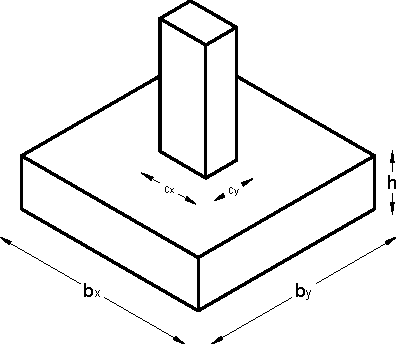
\includegraphics[scale=0.75]{padcad}
	\caption{Μεμονωμένο ορθογωνικό πέδιλο σταθερού ύψους}
	\label{fig:pad}
\end{figure}

\section{Δεδομένα}
Τα δεδομένα (\textlatin{input}) του προβλήματος παρουσιάζονται στους πίνακες που ακολουθούν και αφορούν τα γεωμετρικά χαρακτηριστικά του υπό μελέτη συστήματος, τα μηχανικά χαρακτηριστικά των χρησιμοποιούμενων υλικών και του εδάφους θεμελίωσης και τα εντατικά μεγέθη στο κέντρο βάσης του πεδίλου. Όπου $t_{\varepsilon\delta}$ το βάθος θεμελίωσης και $d$ το στατικό ύψος του πεδίλου.
\begin{table}[H]
\en
\centering
\begin{tabular}{| c | c | c | c | c | c | c | c | c |}
\hline
$b_x$ & $b_y$ & $h$ & $d$ & $t_{\varepsilon\delta}$ & $c_x$ & $c_y$ & $a_x$ & $a_y$ \\
\hline
$2.3$ & $2.3$ & $0.6$ & $0.55$ & $1.0$ & $0.6$ & $0.4$ & $0$ & $0$ \\
\hline
\end{tabular}
\el
\caption{Γεωμετρικά χαρακτηριστικά συστήματος - διαστάσεις σε (\textlatin{m})}
\label{tab:geometry}
\end{table}

\begin{table}[H]
\en
\centering
\begin{tabular}{| c | c | c |}
\hline
$M_x(KNm)$ & $M_y(KNm)$ & $N_{tot}(KN)$ \\
\hline
$550$ & $180$ & $1200$ \\
\hline
\end{tabular}
\el
\caption{Εντατικά μεγέθη στο κέντρο βάσης του πεδίλου}
\end{table}

\begin{table}[H]
\en
\centering
\begin{tabular}{| c | c | c | c |}
\hline
${\gamma}_{\sigma\kappa}(KN/m^3)$ & ${\gamma}_{\varepsilon\delta}(KN/m^3)$ & $f_{ck}(MPa)$ & $f_{yk}(MPa)$ \\
\hline
$25$ & $20$ & $25$ & $500$ \\
\hline
\end{tabular}
\el
\caption{Μηχανικές ιδιότητες υλικών}
\end{table}

\section{Στόχος και αντιμετώπιση}
Στόχος είναι ο έλεγχος επάρκειας του ύψους του στοιχείου θεμελίωσης. Αν το αρχικό ύψος δεν προσφέρει ικανοποιητική αντοχή, τότε επιλέγεται νέο. Αυτό διαπιστώνεται διενεργώντας υπολογισμούς με τη χρήση προγραμματισμού σε γλώσσα \textlatin{C++}, αλλά και αναλυτικών σχέσεων με τη χρήση απλής αριθμομηχανής. Τα αποτελέσματα των δύο διαδικασιών, συγκρίνονται τελικά μεταξύ τους, ώστε να επαληθευτεί η σύγκλισή τους.

Για την ομαλότερη αντιμετώπιση του προβλήματος, αυτό δύναται να χωριστεί σε τρία επιμέρους υποπροβλήματα, τα οποία αναπτύσσονται στη συνέχεια και επιγραμματικά έχουν ως εξής.

\begin{itemize}
  \item Έλεγχος σε διάτμηση.
  \item Έλεγχος σε διάτρηση.
  \item Διαστασιολόγηση σε κάμψη.
\end{itemize}
